\documentclass[12pt]{article}

\usepackage{bm, graphicx, amssymb, amsmath, mathtools, float}
\usepackage[margin=1 in]{geometry}
\usepackage{mathtools}
\usepackage{epstopdf}
\usepackage{enumitem}
\usepackage{color}

\newcommand{\ds}{\displaystyle}
\newcommand{\B}[1]{{\bm #1}}
\newcommand{\U}[1]{{\hat{\bm #1}}}
\newcommand{\T}{^{\mbox{\tiny T}}}
\newcommand{\dd}{\; \text{d}}

%\thispagestyle{empty}

\begin{document}

\newif\ifsolution % Declaration, defaults to false

%% Comment out this line to hide solutions
% \solutiontrue

\begin{center}{\bf AERO-222: Introduction to Aerospace Computation - Spring 2023\\ Homework \#2 - Due Date: Thursday, 9 March, 2023} \vspace{0.5cm}

\textbf{\underline{Show all work and justify your answers!}} \vspace{0.5cm}
\end{center}

{\Large \textbf{Instructions}}
\begin{itemize}
	\item \textit{This homework contains both handwritten and coding problems and shall be submitted according to the following guidelines.}
	\item \textit{Hardcopy:}
	\begin{itemize}
	 \item \textit{Due on CANVAS at 11:59 PM on the day of the deadline.}
	 \item \textit{Shall include screenshots of any hand-written work.}
	 \item \textit{For coding problems, the hardcopy shall include any relevant derivations and emphasize the final results (i.e. boxed, highlighted, etc.). INCLUDE ALL CODING RESULTS (including plots, final values) IN THE HARDCOPY.}
	 \item \textit{Shall be submitted as a single file according to the provided template with the following naming scheme:} ``LastNameHW\#.pdf"
	 \item \textit{If preferable, you can put all of your work into a single Jupyter notebook (.ipynb) with photos of your hand-written work as well. Markdown allows for images. }
	\end{itemize}
	\item \textit{Coding Submission:}
	\begin{itemize}
	 \item \textit{Due on CANVAS at 11:59 PM on the day of the deadline.}
	 \item \textit{Shall be submitted as a single file according to the provided template with the following naming scheme:} ``LastNameHW\#.py" or ``LastNameHW\#.ipynb".
	 \item \textit{The script shall print out all outputs asked for in the problem}.
	\end{itemize}
 \item \textit{Late submissions will be accepted with a 10 point deduction per day late.}
\end{itemize}
\hrulefill

\begin{description}
%%%%%%%%%%%%%%%%%%%%%%%%%%%%%%%%%%%%%%%%%%%%%%%%%%%%%%%%%%%%%%
\item[1. Newton's Method \color{red} (Coding Problem) \color{black} (30 pts).] Apply the Newton's method to find the solution to the equation, $\tan^{-1} x = x^2 - e^{x}$, using $x_0 = 0$ as initial guess.
\begin{enumerate}[label=\textbf{(\alph*)}]
    \item For the convergence criteria, use the residual tolerance, $| f(x_k) | < \varepsilon_y = 10^{-8}$. Report the final residual of your solution and the number of iterations (starting at $i = 1$).
    \item For the convergence criteria use, $| x_{k+1} - x_k | > | x_k - x_{k-1} |$. Report the final error, $\varepsilon_x = | x_{k+1} - x_k |$, and number of iterations. The final error should be the last recorded error above machine precision ($\varepsilon_{x,final} \neq 0$)
    \item Plot the range of convergence for Newton's method.
    \item Compute the order of convergence ($\alpha$) and the asymptotic error constant ($\lambda$) based on your results from part \textbf{b}.
\end{enumerate}

\ifsolution
\color{red}
\textbf{Solution:} \\
\begin{enumerate}[label=\textbf{(\alph*)}]
    \item $N_{\varepsilon_{y}} = 4 \\
    \varepsilon_{y} = f(x_N) \approx 8.32667 \times 10^{-17}$ \\
    \item $N_{\varepsilon_{x}} = 5 \\
    \varepsilon_{x} = \left|x_{N}-x_{N-1}\right| \approx 5.55112 \times 10^{-17}$ \\
    \item
\end{enumerate}
\begin{figure}[H]
    \centering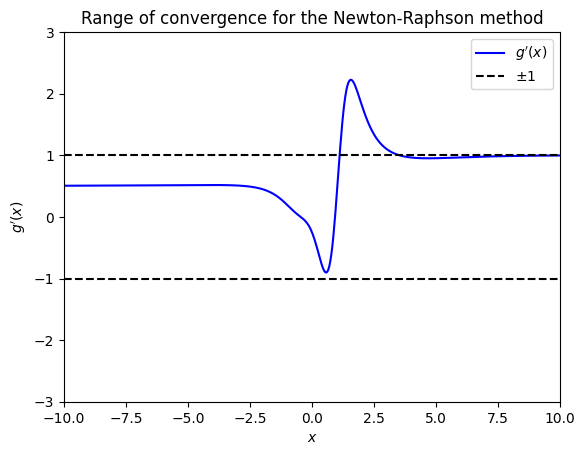
\includegraphics[width=4.5in]{HW2-P1.PNG}
    \caption{Range of convergence}
    \label{fig:Convergence}
\end{figure}

\begin{enumerate}[label=\textbf{(d)}]
    \item $\alpha \approx 1.9573$ \\
    $\lambda \approx 0.11059$ \\
\end{enumerate}
\color{black}
\fi


\item[2. Error Propagation (20 pts).] Consider the following two statements,
\begin{align*}
    z &= 2 x - y + \sin(x y^2) \\
    w &= e^z - 2 (z^2 - 1)
\end{align*}
with mean values $\mu_x = 3$ and $\mu_y = 2$, and standard deviations $\sigma_x = 0.02$ and $\sigma_y = 0.01$. Estimate the following parameters using five significant digits: 
	\begin{enumerate}[label=\textbf{(\alph*)}]
	\item $\mu_w$
	\item $\sigma_w$
	\end{enumerate}

    \color{red}
    \ifsolution
    {\bf Solution}:\\
    \begin{enumerate}[label=\textbf{(\alph*)}]
    
    \item 
    \begin{align*} 
        \mu_z = 2 \mu_x - \mu_y + \sin(\mu_x \, \mu_y^2) = 3.4634\\
        \mu_w = e^{\mu_z} - 2 (\mu_z^2 - 1) = 9.9355
    \end{align*}
    
    \item Partial derivatives:
    \begin{align*}
      \frac{\partial z}{\partial x}\Bigr\rvert_{\mu_x,\mu_y} &= 2 + \mu_y^2 \, \cos(\mu_x \mu_y^2) = 5.3754 \\
      \frac{\partial z}{\partial y}\Bigr\rvert_{\mu_x,\mu_y} &= -1 + 2\mu_x \mu_y \, \cos(\mu_x \mu_y^2) = 9.1262 \\
      \frac{\partial w}{\partial z}\Bigr\rvert_{\mu_z} &= e^{\mu_z} - 4z = 18.072;
    \end{align*}
    Then, the standard deviation of $z$ becomes,
        \begin{equation*}
      \sigma_z = \sqrt{\frac{\partial z}{\partial x}\Bigr\rvert_{\mu_x,\mu_y}^2 \, \sigma_x^2 + \frac{\partial z}{\partial y}\Bigr\rvert_{\mu_x,\mu_y}^2 \, \sigma_y^2} = 0.14102
    \end{equation*}
    and the standard deviation of $w$ is,
        \begin{equation*}
      \sigma_w = \sqrt{\frac{\partial w}{\partial z}\Bigr\rvert_{\mu_z}^2 \, \sigma_z^2} = 2.5486
    \end{equation*}
    
    \end{enumerate}
    \fi
    \color{black}

%%%%%%%%%%%%%%%%%%%%%%%%%%%%%%%%%%%%%%%%%%%%%%%%%%%%%%%%%%%%%%
\item[3. Gaussian Elimination (20 pts).] Use Gaussian Elimination with scaled partial pivoting to solve the following system of equations:
 \begin{equation*}
 \begin{aligned}
    3x_1 - 4x_3 &= -3 \\
    4x_1 + x_2 + 3x_3 &= 8 \\ 
    x_1 - 3x_2 + 5x_3 &= 2 \\ 
 \end{aligned}
 \end{equation*}

 \ifsolution
 \color{red}
 {\bf Solution:}\\

There are a number of different orders of operations, but by rearranging the augmented matrix and substituting back $x_3$ and $x_2$ and $x_1$, the solution is:
$$x_1 \approx 0.65957$$
$$x_2 \approx 1.62766$$
$$x_3 \approx 1.24468$$
 
\color{black}
\fi


%%%%%%%%%%%%%%%%%%%%%%%%%%%%%%%%%%%%%%%%%%%%%%%%%%%%%%%%%%%%%%
\item[4. An Aerospace Application \color{red} (Coding Problem) \color{black} (30 pts).] The following question brings together elements from multiple methods we've covered so far. An Airbus A320 is flying at Mach 0.78. It's Pitot tubes, shown in Figure \ref{fig:Pitot}, measure the total, or stagnation, pressure (pressure when the air hits and is stopped by the tube) as well as the static free-stream pressure.

\begin{figure}[H]
	\centering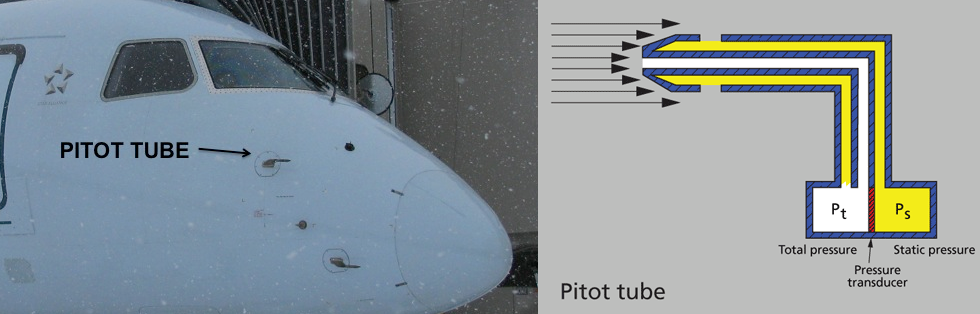
\includegraphics[width=4.5in]{pitot.PNG}
	\caption{Pitot-Static Tubes: Used to measure the ratio of total pressure to static pressure for determining aircraft airspeed.}
	\label{fig:Pitot}
\end{figure}

The ratio of total to static pressure is determined to be: $p_0/p = 1.364$. The following equation relates this change in pressure to the inlet Mach number, $M$, and $\gamma$, the heat capacity ratio:

\begin{equation*}
\dfrac{p_0}{p}= \left[ 1 + \dfrac{\gamma-1}{2}M^2 \right]^{\gamma/(\gamma-1)}
\end{equation*}

Based on the given pressure ratio and Mach number, determine the value of $\gamma$ that satisfies this equation to \emph{four significant figures} of accuracy. State the method and parameters you used (i.e., Fixed-point method, $g(x) = ?$, initial guess = ?, etc.). Also state how many iterations it took and give your final solution estimate. \textbf{Hint:} Don't try to solve analytically for $\gamma$. It might be helpful to plot the function $f(\gamma)$ over a range of values to help you pick a good initial first guess. Choose from any of the iterative methods learned in class to solve.

\ifsolution
\color{red}
\textbf{Solution:} \\
First, rearrange the equation so that it equates to zero:
\begin{equation*}
f(\gamma) = 0 = \left[ 1 + \dfrac{\gamma-1}{2}M^2 \right]^{\gamma/(\gamma-1)} - \dfrac{p_0}{p}
\end{equation*}

A few different methods are possible to find the root. I found the solution using both implementations of Newton's method from problem 1 to showcase two possible solutions. The derivative was approximated using finite differences with h = 1e-9. While the number of iterations may vary depending on the method, all solutions should yield fairly similar results. \\


Error Tolerance: $\varepsilon_{f} = 1 \times 10^{-8}$ \\
Finite Difference: $h=~1e-9$ \\
Initial Guess: $\gamma_{0} = 0$ \\
Given Parameters: $M = 0.7, \ p_0/p = 1.364$ \\

\textbf{Results from Newton's Method:}
\begin{enumerate}[label=\textbf{(\alph*)}]
    \item Using implementation from Problem 1 part a: \\
    Number of Iterations = 3 \\
    $\gamma = 1.024$ \\
    $f(\gamma) = 8.397 \times 10^{-12}$ \\

    \item Using implementation from Problem 1 part b: \\
    Number of Iterations = 5 \\
    $\gamma = 1.024$ \\
    $f(\gamma) = 2.442 \times 10^{-15}$
\end{enumerate}
\color{black}
\fi

\end{description}
\end{document}